\begin{savequote}[75mm]
Strike hot iron and call forth sparks; strike a man and call forth fury; to shape man or metal to thy will, thou must
strike with force.
\qauthor{Collected Sermons of Carras, Thief by Looking Glass Studios}
\end{savequote}

\chapter{Eksperyment numeryczny}
\newthought{Lorem ipsum dolor sit amet}, consectetuer adipiscing elit. Morbi commodo, ipsum sed pharetra gravida, orci
\section{Metodyka}
W ramach poniższej pracy doktorskiej przeprowadzono szereg eksperymentów
numerycznych przy użyciu autorskiego kodu siatkowego PIERNIK, który opiera się
na:
\begin{itemize}
   \item zachowaczym schemacie numerycznym Relaxing TVD~\cite{jin-xin-95} w
      połączeniu z dzielonym, kierunkowym całkowaniem przestrzennym i czasowym
      przy użyciu algorytmu Runge-Kutta drugiego
      rzędu~\cite{2003PASP..115..303T,2003ApJS..149..447P}.
   \item implementacji wielopłynowości, tj. możliwości symulowania wielofazowego
      ośrodka np. płynu neutralnego i płynu bezciśnieniowego (pył) z
      uwzględnieniem oddziaływań międzypłynowych~\cite{piernik1,piernik2}
   \item solwerze multigridowym pozwalającym efektywnie rozwiązywać paraboliczne
      i eliptyczne równania rożniczkowe, a w szczególności równanie Poissona
      opisujące samograwitację pyłu
   \item solwerze multipolowym pozwalającym na szybkie określenie warunków
      brzegowych dla potencjału grawitacyjnego.
   \item implementacji cylindrycznego układu współrzędnych w postaci
      zachowującej moment pędu~\cite{M07,SO10}.
   \item implementacji algorytmu szybkiego transportu
      eulerowskiego~\footnote{ang. \emph{Fast Advection in Rotating Gaseous Objects --
      FARGO}}~\citep{fargo} w ujęciu wielopłynowym.

\end{itemize}
Ponadto PIERNIK korzysta z algorytmu typu \emph{Constraint Transport}
zapewniającego bezźródłowość ewolucji pola magnetycznego, a także możliwość
wykonywania symulacji przy użyciu siatek adaptywnych~\footnote{ang.
\emph{Adaptive Mesh Refinement -- AMR}}.
\par Obliczenia opisywane w tej pracy zostały przeprowadzone z
wykorzystaniem:

\begin{itemize}
   \item infrastruktury PL-Grid, w szczególności klastrów
      komputerowych Galera+ (TASK), Hydra (ICM), Zeus (ACK CYFRONET), Inula
      (PCSS) w ramach grantu \emph{plggpiernik},
   \item klastrów PRACE, w szczególności klastów komputerowych
      Cartesius (SurfSara), Fionn (ICHEC) w ramach grantu \emph{PIERNIK-SI} w
      projekcie DECI-11
\end{itemize}
Sumaryczne zużycie wyniosło kilka milionów CPUh.


%We conduct numerical simulations with the aid of a
%parallel MHD code PIERNIK using the cylindrical coordinate system. 
%Following
%\cite{M07} and \cite{SO10} we use ''angular momentum-conserving form'' of the
%$\phi$-momentum equation, which with respect to Cartesian geometry introduces
%only one additional source term to equations~\mref{eq3} - \mref{eq4}:
%$\left((\rho_g u_\phi + P) / R\right)\mathbf{\hat{R}}$ and $(\rho_d w_\phi / R)
%\mathbf{\hat{R}}$ respectively.


\subsection{Podstawowe równania}
Globalna dynamika dysku okołogwiazdowego można opisać poprzez dwa, wzajemnie ze
sobą oddziałujące płyny: neutralny gaz podlegający izotermicznemu równaniu
stanu oraz pył jako bezciśnieniowy płyn. Równania hydrodynamiki przyjmują dla
takiego modelu następującą postać:

% CONSERVATIVE FORM
\begin{align}
\partial_t \rho_g &+ \nabla\cdot\left(\rho_g\mathbf{u}\right) = 0,\\
\partial_t \rho_d &+ \nabla\cdot\left(\rho_d\mathbf{w}\right) = 0,\\
\partial_t \left(\rho_g\mathbf{u}\right) &+
   \nabla\cdot(\mathbf{u}\otimes(\rho_g\mathbf{u})+P) \notag\\
 &= -\rho_g\left(\nabla\Phi +
\frac{\rho_d}{\tau_f\rho_g}(\mathbf{u}-\mathbf{w})\right),\label{eq3}\\
\partial_t \left(\rho_d\mathbf{w}\right) &+
\nabla\cdot(\mathbf{w}\otimes(\rho_d\mathbf{w})) \notag\\
 &= -\rho_d\left(\nabla\Phi + \frac{1}{\tau_f}(\mathbf{w}-\mathbf{u})\right)
\label{eq4}.
\end{align}
% NON-CONSERVATIVE FORM
%\begin{align}
%\partial_t \rho_g &+ \nabla\cdot\left(\rho_g\mathbf{u}\right) = 0,\\
%\partial_t \rho_d &+ \nabla\cdot\left(\rho_d\mathbf{w}\right) = 0,\\
%\partial_t \mathbf{u} &+ \left(\mathbf{u}\cdot\nabla\right)\mathbf{u} = 
% -\nabla\Phi + \frac{\rho_d}{\tau_f\rho_g}(\mathbf{w}-\mathbf{u})
% -c_s^2\nabla\ln\rho_g,\label{eq3} \\
%\partial_t \mathbf{w} &+ \left(\mathbf{w}\cdot\nabla\right)\mathbf{w} = 
% -\nabla\Phi - \frac{1}{\tau_f}(\mathbf{w}-\mathbf{u}),\label{eq4}
%\end{align}

\noindent gdzie $\rho_g$, $\rho_d$ to odpowiednio gęstości gazu i pyłu,
$\mathbf{u}$, $\mathbf{w}$ ich prędkości, $P$ to ciśnienie gazu, $\tau_f$ jest
skalą czasową tarcia~\footnote{ang. friction time}~\mref{eq:tauf}, a $\Phi$ to
potencjał grawitacyjny. Celem pracy jest wyizolowanie niestabilności
strumieniowej z pośród szeregu innych procesów, które mogą zachodzić w powyższym
modelu. Z tego względu zaniedbano pionową składową przyspieszenia grawitacyjnego
pochodzącą od centralnego obiektu w dysku, która prowadziła by do naturalnej
sedymentacji pyłu w płaszczyźnie dysku i wzbudzenia się niestabilności
Kelvina-Helmholtza~\cite{JHK06}.

%W ramach pracy skupiono się na dyskach rozciągających się relatywnie dużych
%promienii tj. 2~AU. Zakładając, za pracą~\cite{CD93}, że przejście do
%reżimu Stokesa zachodzi dla ziaren pyłu o promieniu większym niż
%$a = 9/4\lambda_g$ gdzie $\lambda_g = 4.2\times 10^4\textrm{
%cm} (10^{-14}\textrm{ g cm}^{-3}/\rho_g) \approx (R/1 \textrm{AU})^{2.75}$~cm 
%jest średnią drogą swobodną molekuł gazu~\citep{W77,BT09}, zaś $R$ jest
%odległością radialną od centrum dysku. Przy tych założeniach, reżim Epstein ma
%%zastosowanie dla dominującej części domeny obliczeniowej nawet dla największych
%symulowanych przez nas ziaren pyłu. Skala czasowa tarcia przyjmuję zatem
%następującą postać:
%
\begin{figure*}
   \centering
   \begin{tabular}{@{}cc@{}}
      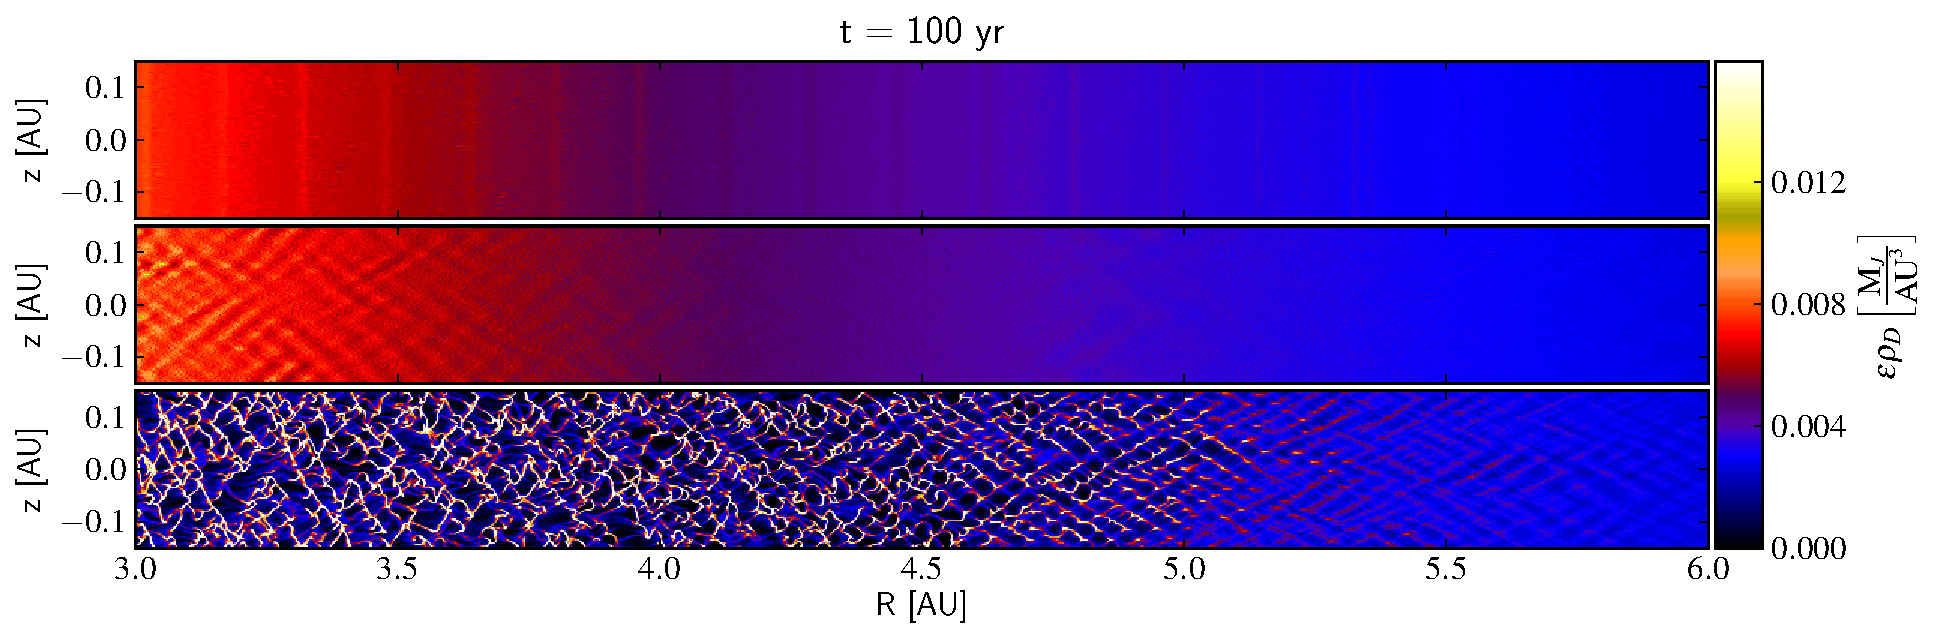
\includegraphics[width=0.49\linewidth]{figures/fig1a} & 
      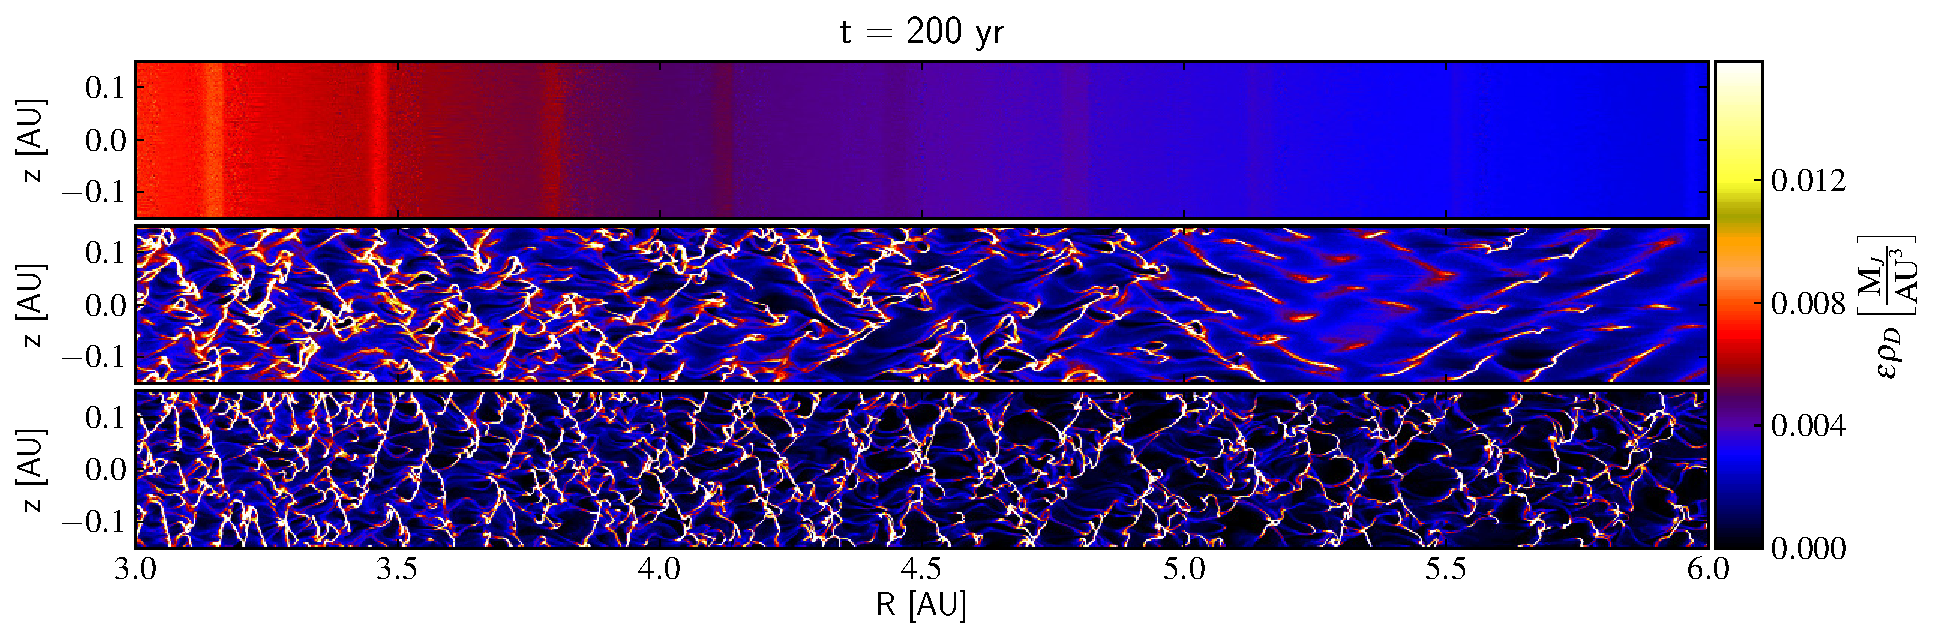
\includegraphics[width=0.49\linewidth]{figures/fig1b} \\
      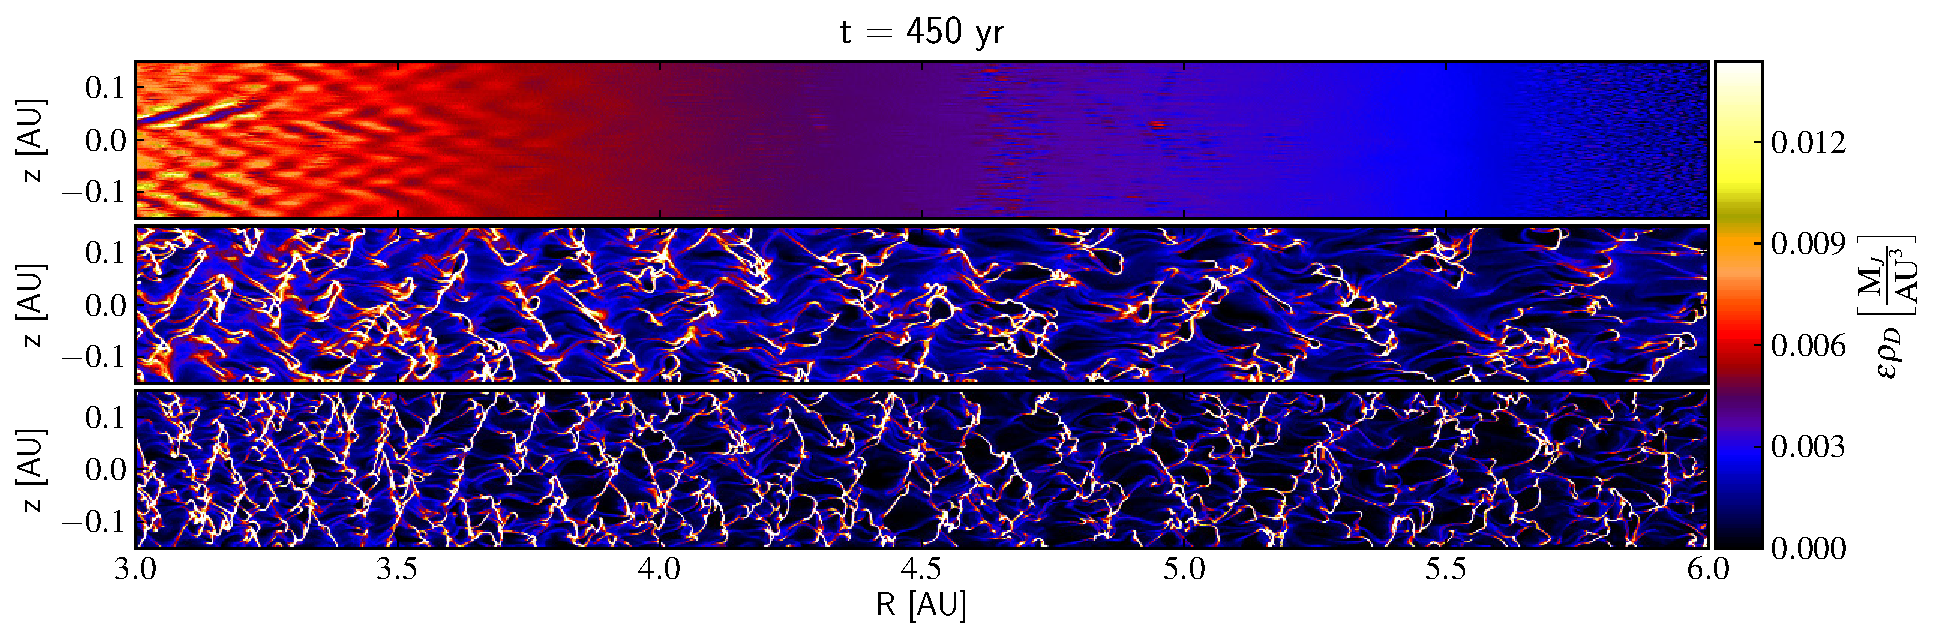
\includegraphics[width=0.49\linewidth]{figures/fig1c} &
      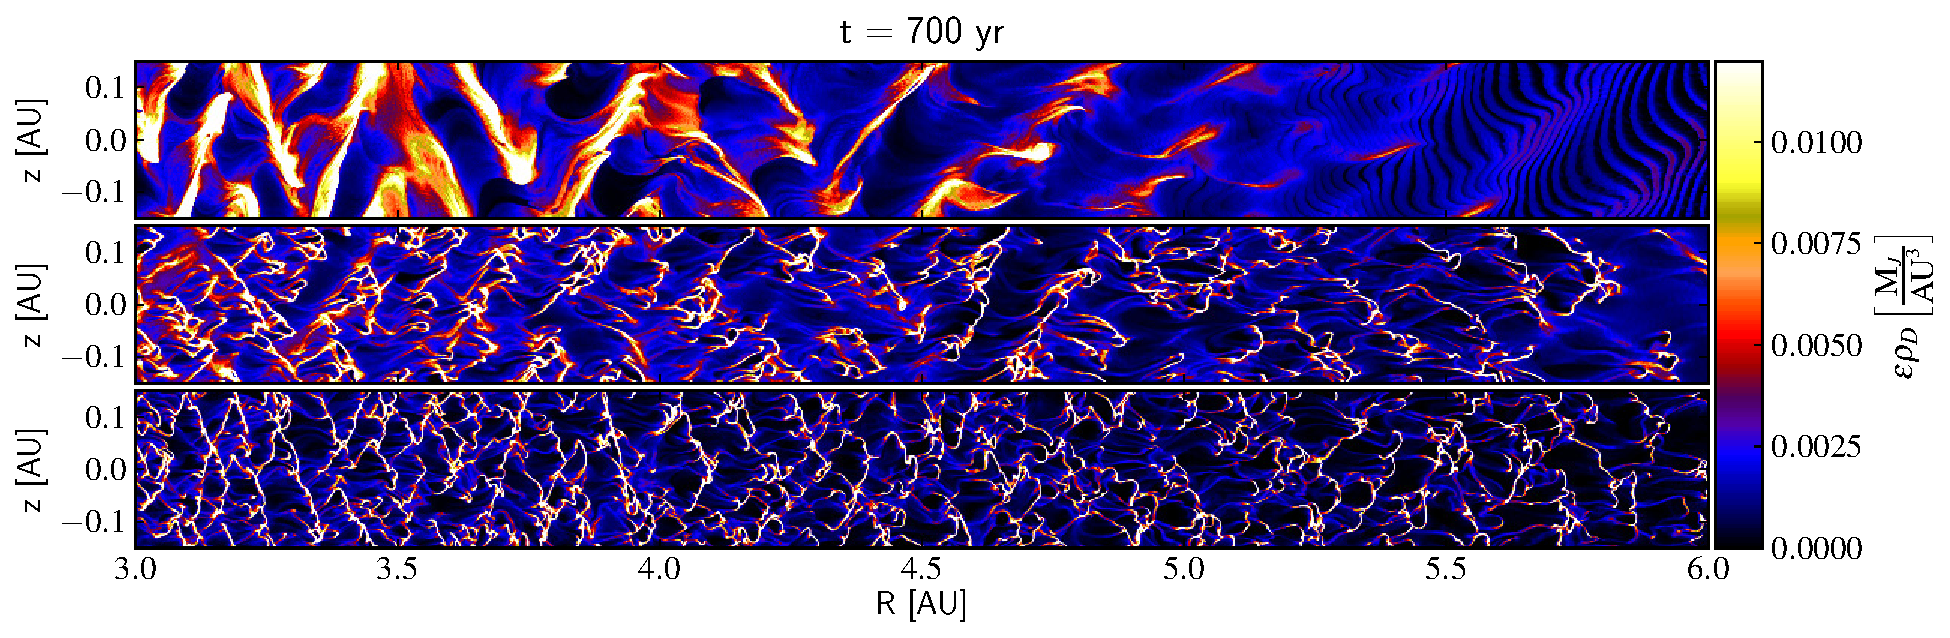
\includegraphics[width=0.49\linewidth]{figures/fig1d}
   \end{tabular}
   \caption{Migawki gęstości pyłu dla symulacji z $50$~cm ziarnami pyłu
      dla czasu $100$, $200$, $450$ oraz $700$~lat odpowiednio dla lewego
      górnego, prawego górnego, dolnego lewego i dolnego prawego panelu.
      Każdy z paneli jest podzielony na trzy części różniące się początkowym 
      $\epsilon = 0.2, 1, 2.0$ odpowiednio dla górnego (BAh), środkowego (BB) i
      dolnego (BC) podpanelu.}
   \label{fig1}
\end{figure*}
%
\subsection{FARGO}
Ze względu na obecność rotacji, dyski keplerowskie stanowią mało wdzięczny
obiekt badań numerycznych, szczególnie w wypadku kiedy charakterystyczne
prędkości płynu osiągane w interesujących procesach są drobnym ułamkiem
prędkości rotacji. Zgodnie z warunkiem Couranta-Friedrichsa-Lewy'ego, stabilność
schematu numerycznego jest zapewniona wtedy i tylko wtedy, kiedy w jednym kroku
całkowania numerycznego sygnał nie propaguję się dalej niż o jedną komórkę
obliczeniową. W związku z tym, że zarówno prędkość rotacji dysku keplerowskiego
jak i azymutalny rozmiar komórki na siatce cylindrycznej jest malejącą funkcją
promienia, to najsilniesze ograniczenie na rozmiar kroku czasowego wprowadza
dynamika gazu na najkrótszej symulowanej orbicie. Jedną z technik pozwalających
uniknąć powyższych więzów jest algorytm FARGO~\citep{Masset00}. Oryginalnie
został on zaprojektowany dla dwuwymiarowych dysków, lecz został rozszerzony
przez innych autorów~\cite{fargo2} do przypadków trójwymiarowych. Poniższa praca
rozwija go w kontekście wielu płynów.

\par FARGO opiera się na kierunkowym podziale części adwekcyjnej równań
hydrodynamiki. W kierunku radialnym i wertykalnym stosuje się klasyczny solwer
(w przypadku PIERNIKa RTVD), natomiast w kierunku azymutalnym rozbija się
adwekcję na trzy etapy:
\begin{enumerate}
   \item obliczenie średniej prędkości kątowej $\bar{\omega}_i$ dla każdego
      płynu i każdego promienia o indeksie $i$
      \begin{equation}
         \bar{\omega}_i = \frac{1}{N_\varphi~N_z} ~ \sum_{j,k} \omega_{i,j,k},
      \end{equation}
      gdzie $N_\varphi,\,N_z$ to odpowiednio liczba komórek w kierunku
      azymutalnym i wertykalnym.

   \item  obliczenie całkowitej liczby komórek dla przesunięcia w kierunku
      azymutalnym
      \begin{equation}
         n_i = {\tt Nint} \left( \bar{\omega}_i \Delta t/\Delta \varphi \right),
      \end{equation}
      gdzie {\tt Nint} oznacza funkcję określającą \emph{najbliższą liczbę
      całkowitą}. Co można wyrazić jako ,,prędkość przesunięcia''
      \begin{equation}
         \omega_i^{\rm SH} = n_i \frac{\Delta \varphi}{\Delta t}.
      \end{equation}
   \item obliczenie stałej wartości prędkości ,,rezydualnej'' dla każdego
      promienia
      \begin{equation}
         \omega_i^{\rm cr}= \bar{\omega}_i - \omega_i^{\rm SH}
      \end{equation}
   \item obliczenie właściwej prędkości ,,rezydualnej'' dla każdej komórki
      \begin{equation}
         \omega_{i,j,k}^{\rm res} = \omega_{i,j,k} - \bar{\omega}_i
      \end{equation}
\end{enumerate}

Powyższe cząstkowe prędkości kątowe sumują się do wyjściowej prędkości dla
poszczególnych komórek

\begin{equation}
   \omega_{i,j,k} = \omega_{i,j,k}^{\rm res} + \omega_i^{\rm cr} + \omega_i^{\rm SH}.  
\end{equation}

Adwekcja jest następnie wykonywana w trzech krokach, odpowiednio dla każdej
prędkości kątowej $\omega_i^{\rm SH}, \omega_i^{\rm cr}, \omega_{i,j,k}^{\rm
res}$: ostatnie dwie prędkości przyużyciu oryginalnego algorytmu numerycznego
(RTVD), zaś $\omega_i^{\rm SH}$ poprzez zwykłe przesunięcie wartości płynowych o
całkowitą liczbę komórek. Korzystąc z faktu, że $\omega_i^{\rm SH} \gg
\max\left(\omega_i^{\rm cr}, \omega_{i,j,k}^{\rm res}\right)$, a tylko prędkości
po prawej stronie nierówności mają wpływ na warunek CFL, w znaczący sposób
zwiększamy krok czasowy. Co prawda, aby zachować stabilność algorytmu należy
zapewnić że przesunięcie w kierunku azymutalnym nie odseparuje dwóch sąsiędnich
(w kierunku radialnym i wertykalnym) komórek, co przekłada się na warunek

\begin{equation}\label{eq:tshear}
   \Delta t_{\rm shear} = 0.5 ~ \min_{i,j,k} \left( \frac{\Delta\varphi}
   {|\omega_{i,j,k} - \omega_{i-1,j,k}|} \right)
\end{equation}

Niemniej jednak pomimo ograniczenia~\mref{eq:tshear}, dla typowych eksperymentów
numerycznych przeprowadzonych w tej pracy zastosowanie FARGO pozwolilo uzyskać
od 10 do 100 krotnego wydłużenia kroku czasowego.

\subsection{Schemat implicit dla oddziaływania}
Both components i.e. gas and dust are treated as fluids~\citep{piernik2} which
are dynamically coupled via the friction force. In order to prevent large
timestep constraint from drag force acceleration we used the semi-implicit
scheme by~\cite{TB09}. We allow the system to relax numerically (during the
period of initial $10$~yrs of the simulation) before we ''turn on'' the
aerodynamic drag force and seed dust velocities with low--amplitude random
noise. The feedback of the linear drag force scales with the density ratio of
dust to gas $\epsilon\equiv \rho_d/\rho_g$.

\subsection{Potencjał grawitacyjny}
\section{Warunki początkowe}
The initial density profile for gas roughly follows prescription of Minimal Mass
Solar Nebula~\citep{H81}
\begin{equation}
   \Sigma(R) = 1700 \left(\frac{R}{1\textrm{ AU}}\right)^{-3/2} 
   \textrm{ g cm}^{-2}.
\end{equation}
We assume isothermal equation of state and a constant temperature $T_0 = 170$~K
across the whole disc. 
We assume gravitational field from a point mass $M=1\,\textrm{M}_\odot$, and
neglect the vertical component of gravitational acceleration towards the central
mass, implying no vertical stratification of the disc. Yet, we refer to the
vertical scaleheight $H$ to estimate  volume density of gas at given radius,
relying on the hydrostatic equilibrium density distribution in the presence of
the vertical gravity of a point mass
%
\begin{equation}
   \rho(R,z) =  \rho(R,0) \exp\left(-\frac{z^2}{2H(R)^2}\right),
\end{equation}
where $\rho(R,0)$ is gas density at the disc midplane and $H^2 = 2 c_s^2 R^3/
GM$.
%
The surface gas density is given by
\begin{equation}
   \Sigma(R) = \int_{-\infty}^\infty \rho(R,z) dz,
\end{equation}
%
The corresponding value of midplane gas density is
\begin{equation}
   \label{eq:rho}
    \rho(R,0) = \frac{\Sigma(R) }{\int_{-\infty}^\infty
   \exp\left(-\frac{z^2}{2H(R)^2}\right) dz}.
\end{equation}
For the chosen disc temperature $T_0$ the integral on the right hand side of
\mref{eq:rho} varies from $0.4$~AU to $2.0$~AU over the range of radii $R\in
[2,6]$~AU. 
We assume for simplicity its value equal to $1$~AU. 

We assume the vertical extent of the computational domain $L_z = 0.3$~AU, and
impose periodic boundary conditions at upper and lower $z$-boundaries. The
initial condition relies on a radial force balance for the gas and dust
components independently. The gas component remains in a hydrostatic equilibrium
resulting from the radial balance of gravity, centrifugal and pressure forces,
while the pressure gradient term is absent in the equation of motion for the
dust component.  Reflecting boundary conditions are set on the inner and outer
boundaries of the computational grid to prevent mass escape from the
computational domain. 

\par To minimise unphysical wave reflections, we implement wave killing zones
close to the inner and outer radial boundaries. The inner wave killing zones
cover 0.5 AU near the inner and outer edges of the computational domain. In
these zones, we add an additional damping term, in the evolution equations of
each fluid variable

\begin{equation}
  \frac{\textrm{d}X}{\textrm{d}t} = - \frac{X-X_0}{T_d}f(R),
\end{equation}
together with
\begin{equation}
   \begin{split} 
      f(R) &= 1 - \tanh\left(\left(R - R_\textrm{in} + 1
      \right)^{f_\textrm{in}}\right)\\ &+ \max\left\{ \tanh\left(\left(R -
      R_\textrm{out} + 1\right)^{f_\textrm{out}}\right), 0\right\}, 
   \end{split}
\end{equation}
where $X_0$ is the initial value of $X$ and $T_d$ is the damping timescale. We
chose $T_d$ of the order of orbital period.  The exponents
$f_\textrm{in}=f_\textrm{out}=10$ control the width of the transition layer
between the unmodified to the damped zones. Within the damped zones, the effects
of undesired wave reflection are essentially minimised.
%
\subsection{Simulation parameters}
%
We have performed a parameter sweep for the ratio of dust to gas density
$\epsilon$ and the size of particles $a$, at two different resolutions of the
computational grid in 2D, and additionally we have realized one of the models in
3D. Our choice of these parameters follows closely that of JY07, to enable
detailed comparison of the results.

The full list of simulations together with their main parameters is presented in
Table~\ref{tab1}. In all simulations the domain has height of $0.293$~AU,
for 2D it covers radii from 2 to 7~AU, whereas BB3D extends from 2 to 12~AU and
spans $\varphi\in[0, \pi/6]$.  Following JY07 we vary $\epsilon$ from 0.2 to
2.0~in order to exhibit morphologically different outcomes of nonlinear phase of
streaming instability.  We choose particle radii to be grater than $10$~cm and
less than $50$~cm so that (1) particles fall into Epstein regime in all
simulations, (2) their size could be plausibly explained by the growth processes
e.g. collisional agglomeration.

\begin{table}
   \centering
   \begin{tabular}{cccccc}
      \hline
      Run & $N_r \times N_\varphi \times N_z$ &
      $a$~[cm] & $\epsilon$ & $T_\textrm{end}$~[yr] \\
      \hline
      BB3D &  $5120  \times 128 \times 150$  & 50  & 1.0 & 500  \\
      AA   &  $5120  \times 1   \times 300$  & 10  & 0.2 & 3000 \\
      AB   &  $5120  \times 1   \times 300$  & 10  & 1.0 & 3000 \\
      AC   &  $5120  \times 1   \times 300$  & 10  & 2.0 & 3000 \\
      BA   &  $5120  \times 1   \times 300$  & 50  & 0.2 & 3000 \\
      BB   &  $5120  \times 1   \times 300$  & 50  & 1.0 & 3000 \\
      BC   &  $5120  \times 1   \times 300$  & 50  & 2.0 & 3000 \\
      AAh  &  $10240 \times 1   \times 600$  & 10  & 0.2 & 1700 \\
      AAu  &  $20480 \times 1   \times 1200$ & 10  & 0.2 & 1800 \\
      ABh  &  $10240 \times 1   \times 600$  & 10  & 1.0 & 1400 \\
      BAh  &  $10240 \times 1   \times 600$  & 50  & 0.2 & 1730 \\
      BBh  &  $10240 \times 1   \times 600$  & 50  & 1.0 & 3000 \\
      \hline
   \end{tabular}
\caption{Simulation parameters. Columns give, from left to right, name of the
   run, span of the computational domain in AU (r,z) and azimuthal angle, grid
   resolution, particle diameter in cm, solids-to-gas ratio, and total run time
   in units of years.} 
\label{tab1}
\end{table}

%%%%%%%%%%%%%%%%%%%%%%%%%%%%%%%%%%%%%%%%%%%%%%%%%%%%%%%%%%%%%%%%%%%%%%%%%%%%%%%%
% vim: tw=80 ts=3: 
